\begin{figure}[t]
\begin{center}
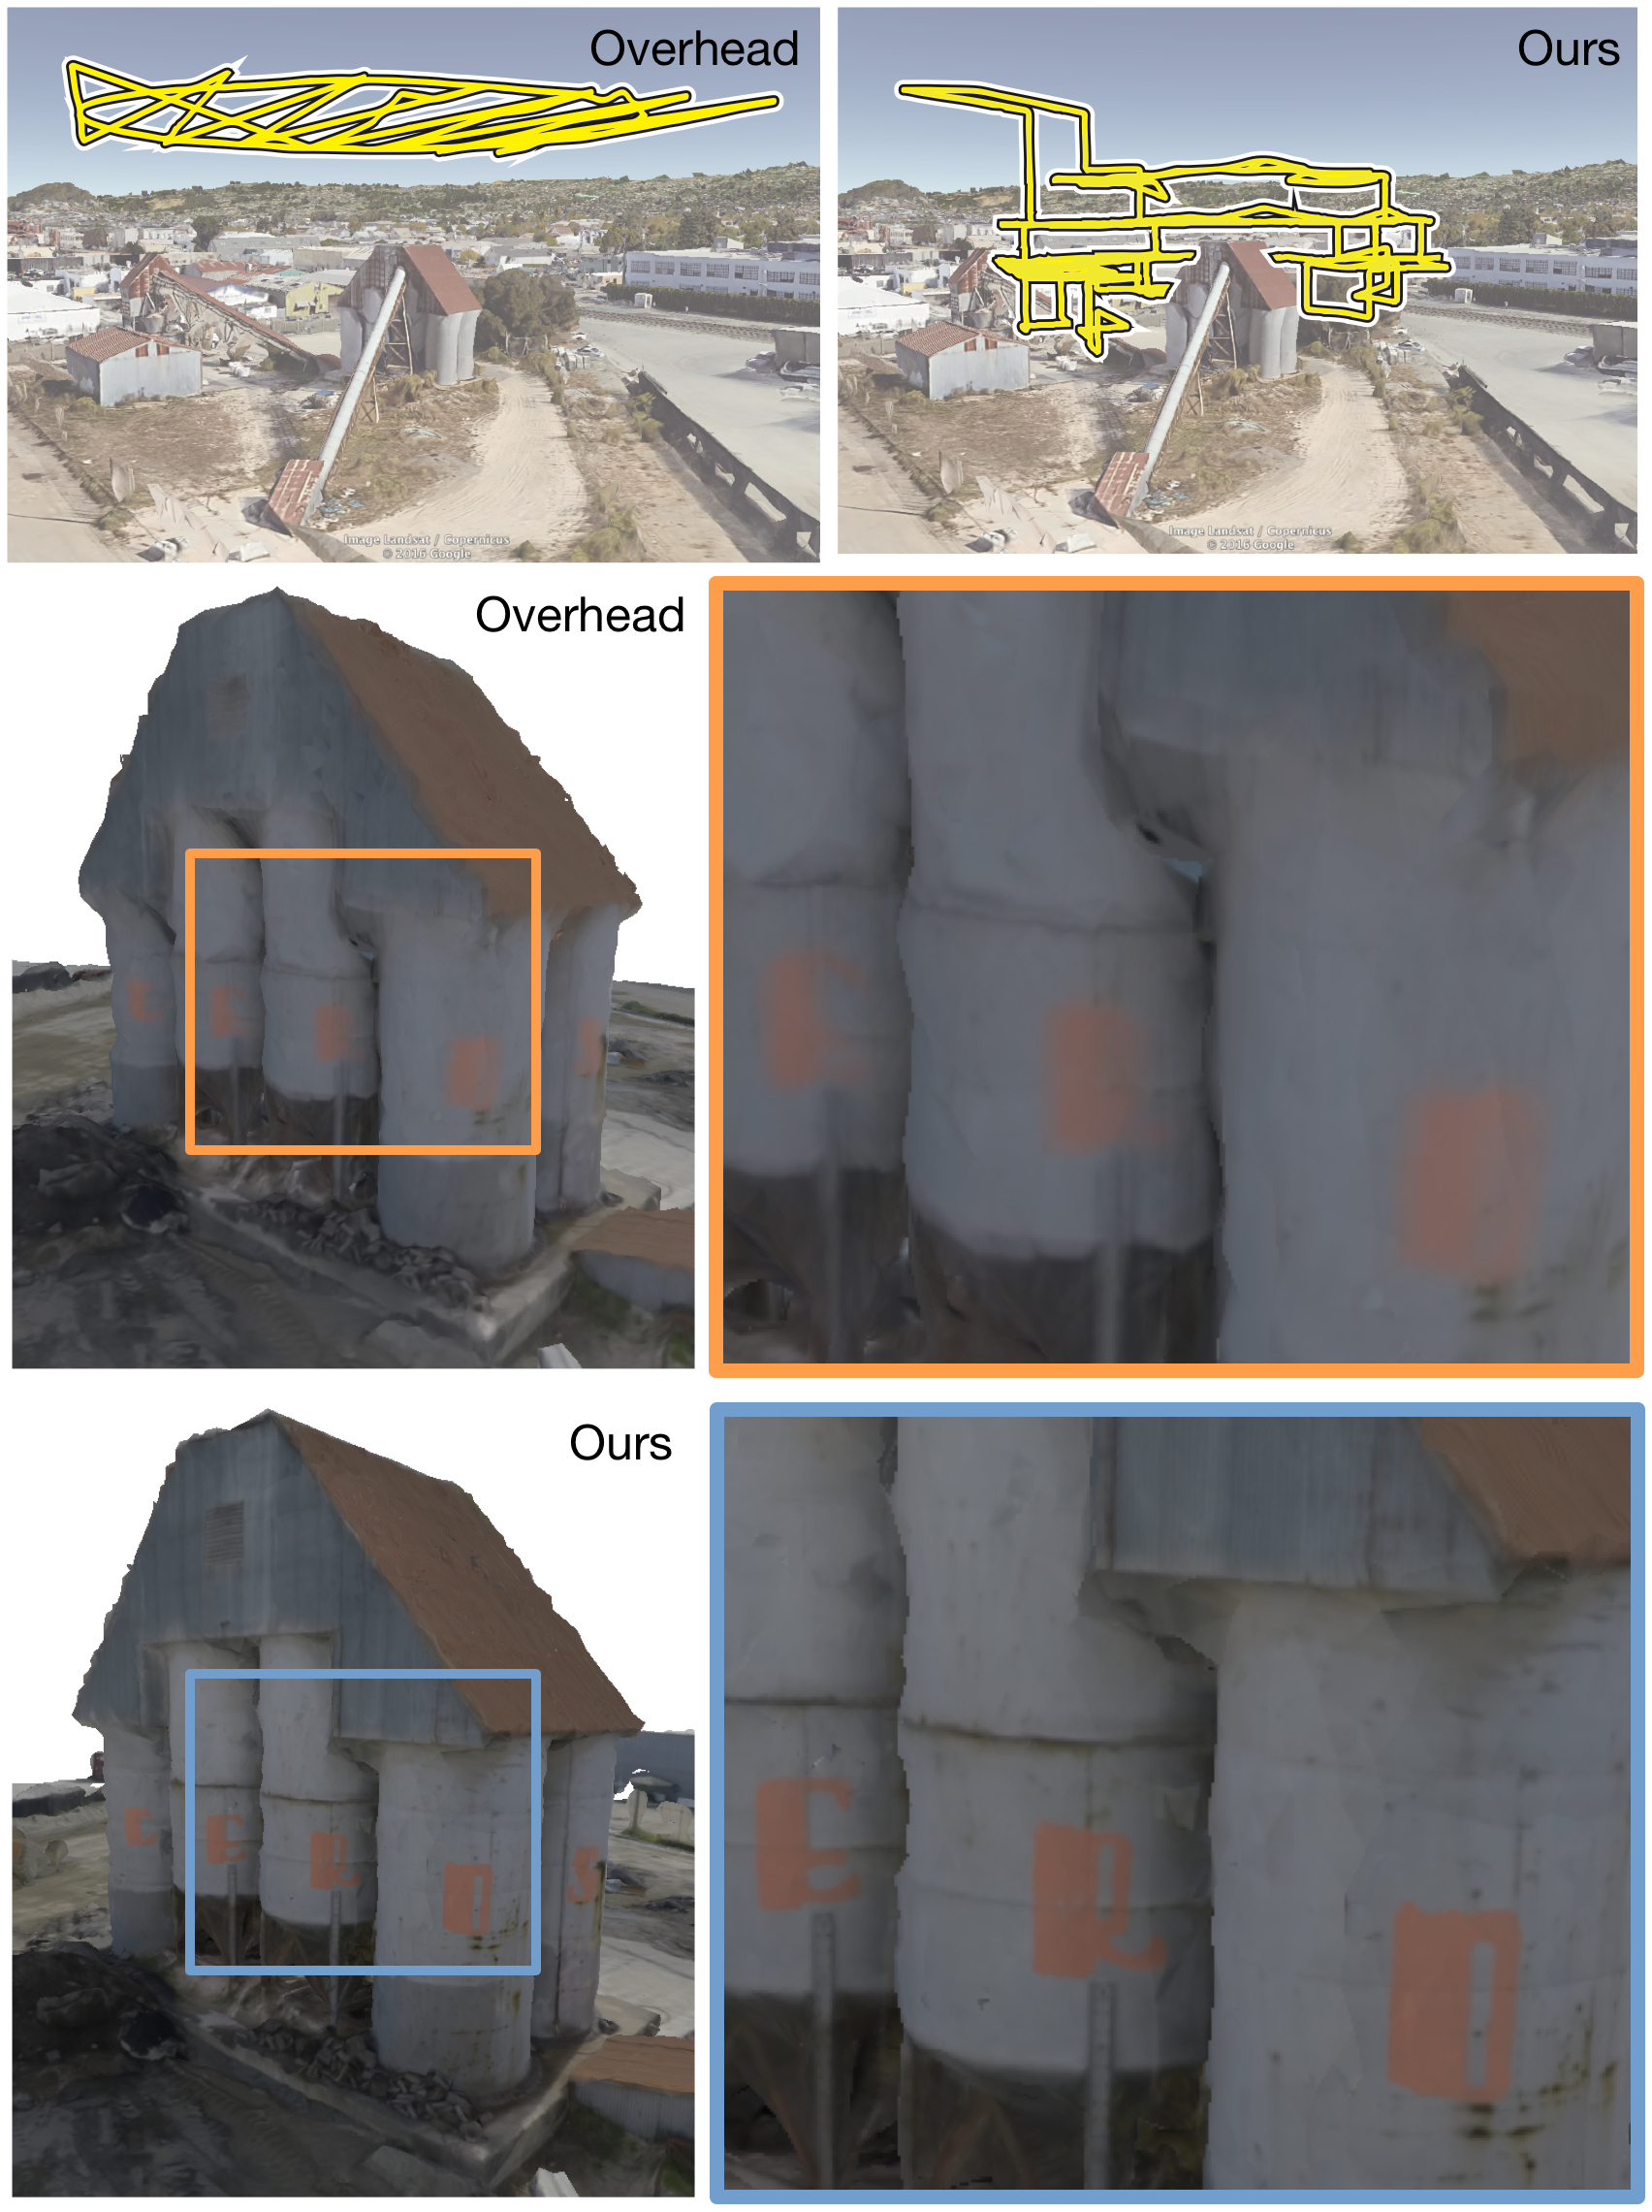
\includegraphics[width=0.47\textwidth]{images/2017_iccv/teaser.jpg}{\vspace{-7pt}}
\end{center}
\caption{
3D reconstruction results obtained using our algorithm for generating aerial 3D scanning trajectories, as compared to an overhead trajectory.
Top row: Google Earth visualizations of the trajectories.
Middle and bottom rows: results obtained by flying a drone along each trajectory, capturing images, and feeding the images to multi-view stereo software.
Our trajectories lead to noticeably more detailed 3D reconstructions than overhead trajectories.
In all our experiments, we control for the flight time, battery consumption, number of images, and quality settings used in the 3D reconstruction.
}
\vspace{-13pt}
\label{fig:teaser}
\end{figure}

\vspace{-16pt}
\section{Introduction}

Small consumer drones equipped with high-resolution cameras are emerging as a powerful tool for large-scale aerial 3D scanning.
In order to obtain high-quality 3D\ reconstructions, a drone must capture images that densely cover the scene.
Additionally, 3D reconstruction methods typically require surfaces to be viewed from multiple viewpoints, at an appropriate distance, and with sufficient angular separation (i.e., baseline) between views.
%These constraints require users to carefully plan trajectories or carefully maneuver the drone which requires experience and skill.
Existing autonomous flight planners do not always satisfy these  requirements, which can be difficult to reason about, even for a skilled human pilot manually controlling a drone.
Furthermore, the limited battery life of consumer drones provides only 10--15 minutes of flight time, making it even more challenging to obtain high-quality 3D reconstructions.

%The proliferation of inexpensive, high quality cameras along increasingly commoditized aerial platforms (drones), have made it easier %to capture and model large 3D environments using structure-from-motion (SfM) and multi-view stereo (MVS) methods.
%However, ensuring a high quality reconstruction with good coverage with reasonable capture and reconstruction times is not trivial.
%The quality of a reconstruction is a function of the number of images, the spacing between the sampled camera poses (baselines), the distance to surfaces in the scene, and the amount of the scene that has been viewed~\cite{hornung:2008}.
%Controlling a drone to optimize these properties is very challenging, even for an experienced pilot, especially given the hard constraints posed by the limited battery life of a drone, which can limit captures to only minutes.
%As a result, drone-based scene capture can require many flights to ensure quality and coverage, or alternatively one must sacrifice quality and coverage.

In lieu of manual piloting, commercial flight planning tools generate conservative trajectories (e.g., a lawnmower or orbit pattern at a safe height above the scene) that attempt to cover the scene while respecting flight time budgets \cite{3dr:2017a,pix4d:2017a}.
However, because these trajectories are generated with no awareness of the scene geometry, they tend to over-sample some regions (e.g., rooftops), while under-sampling others (e.g., facades, overhangs, and fine details), and therefore sacrifice reconstruction quality.

We propose a method to automate aerial 3D scanning, by planning good camera trajectories for reconstructing large 3D scenes (see Figure \ref{fig:teaser}).
Our method relies on a mathematical model that evaluates the usefulness of a camera trajectory for the purpose of 3D scanning.
Given a coarse estimate of the scene geometry as input, our model quantifies how well a trajectory covers the scene, and also quantifies the diversity and appropriateness of views along the trajectory.
Using this model for scene coverage, our method generates trajectories that maximize coverage, subject to a travel budget.
We bootstrap our method using coarse scene geometry, which we obtain using the imagery acquired from a short initial flight over the scene. 

%Subsequently, we fly our optimized trajectory, and we use the additional imagery from our optimized flight to reconstruct the high-fidelity scene during post-processing.
%As our experiments show, this strategy improves the completeness and visual quality of our reconstructed 3D models.

%In particular, our approach is designed to account for the domain-specific requirements of modern 3D reconstruction algorithms, i.e., we aim to maximize the area covered by all camera locations, across all surface points, subject to a budget to account for the limited flying time of a drone. We perform the optimization by bootstrapping with a geometry estimate from a simple short flight that we used to planning a new trajectory. After flying this new trajectory the images acquired are added to the 3D reconstruction process to refining the geometry from the initial short flight, ultimately yielding higher-quality 3D reconstructions than would be possible to obtain otherwise.

We formulate our trajectory planning task as a reward-collecting graph optimization problem known as \textit{orienteering}, that combines aspects of the traveling salesman and knapsack problems, and is known to be NP-hard \cite{gunawan:2016,vansteenwegena:2011}.
However, unlike the additive rewards in the standard orienteering problem, our rewards are non-additive, and globally coupled through our coverage model.
We make the observation that our coverage model exhibits an intuitive diminishing returns property known as \textit{submodularity}~\cite{krause:2014}, and therefore we must solve a \textit{submodular orienteering} problem.
Although submodular orienteering is strictly harder than additive orienteering, it exhibits useful structure that can be exploited.
We propose a novel transformation of our submodular orienteering problem into an additive orienteering problem, and we solve the additive problem as an integer linear program. We leverage submodularity extensively throughout the derivation of our method, to obtain approximate solutions with strong theoretical guarantees, and dramatically reduce computation times.

We demonstrate the utility of our method by using it to scan three large outdoor scenes: a barn, an office building, and an industrial site.
We also quantitatively evaluate our algorithm in a photorealistic video game simulator.
In all our experiments, we obtain noticeably higher-quality 3D reconstructions than strong baseline methods.
% CUTTING TO SHORTEN -- that works well for MVS algorithms.
%
%which we exploit throughout our method to obtain strong approximation guarantees and significantly reduce computation times.

%% THIS FOLLOWING SENTENCE DOES NOT ADD MUCH !
%We evaluate our algorithm quantitatively using a photorealistic game engine and use it to scan three large outdoor scenes. We show that our method consistently recovers more
%complete 3D models with higher resolution texture maps compared to existing methods.

%We demonstrate the utility of our algorithm by using it to scan three large outdoor scenes: a barn, an office building, and an industrial site. We also quantitatively
